The rapid scaling of large language models (LLMs) has placed efficient hardware utilization at the core of modern AI systems~\cite{kaplan2020scaling}. To meet these demands, specialized accelerators such as GPUs and NPUs have become the backbone of large-scale training and inference~\cite{choquette2021nvidia,huawei2019ascend}. At the core of these platforms are kernels that implement fundamental operations, including matrix multiplication and attention, which dominate execution time in LLM workloads. As a result, the end-to-end performance, efficiency, and cost of LLM systems are largely determined by kernel efficiency rather than hardware peak capability. 

% Despite their foundational importance, developing efficient kernels remains a formidable engineering challenge. Achieving near-peak utilization demands deep expertise in both algorithmic structure and hardware-specific details. Moreover, kernel optimization is inherently non-scalable: implementations are often tightly coupled to specific hardware architectures and workload characteristics, making them difficult to reuse or generalize across GPU generations or hardware vendors~\cite{wu2023pytorch}.

Despite their foundational role, the development of efficient kernels remains a formidable engineering challenge. Achieving near-peak hardware utilization requires deep expertise in both algorithmic design and hardware-specific intricacies. Furthermore, kernel optimization is inherently non-scalable: implementations are often tightly coupled to particular hardware architectures and workload characteristics, which hinders their reuse and generalization across different GPU generations or hardware vendors~\cite{wu2023pytorch}.

\begin{figure*}
    \centering
    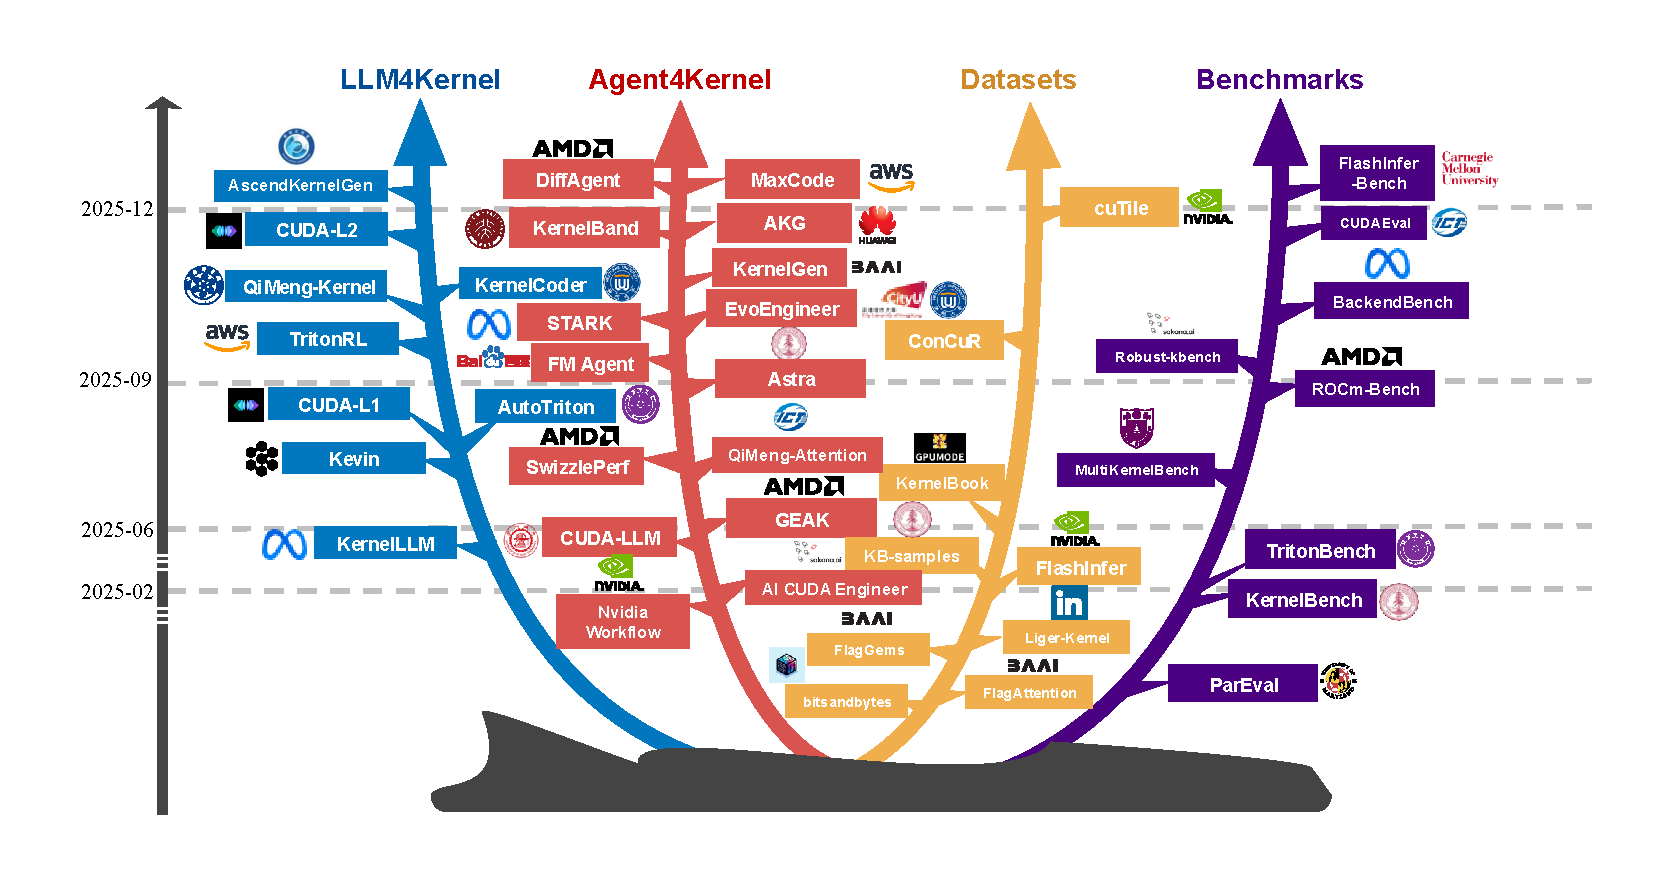
\includegraphics[width=0.85\linewidth]{img_pdf/1_f.pdf}
    \caption{Illustration of the growth trend in the field of LLM-driven kernel generation. We organize these research works chronologically and categorically based on their publication dates and the domains they belong to.}
    \label{fig:1}
\end{figure*}



In response to these challenges, LLMs and LLM-based agents offer a transformative paradigm for kernel generation. By training on vast repositories of code and documentation, LLMs effectively compress expert-level ``world knowledge'' regarding hardware specifications, enabling them to bridge the semantic gap between high-level algorithms and low-level implementation details. Beyond static code generation, LLM-based agents excel in navigating the irregular optimization landscape through iterative refinement. This closed-loop approach not only drastically reduces the engineering but also generalizes across workloads and hardware configurations, toward a future of scalable, automated kernel discovery. As a result, LLMs and LLM-based agents are emerging as compelling foundations for the next generation of kernel generation and optimization frameworks.


Although the integration of LLMs and LLM-based agents into kernel generation marks a rapidly advancing frontier in AI systems research, the absence of a systematic survey has resulted in a fragmented research landscape. This survey addresses this gap by presenting a unified overview of the field, clarifying foundational concepts, and highlighting emergent methodologies and trends. A key contribution is our consolidated resource infrastructure, featuring a structured compilation of training-ready kernel datasets and a literature collection tailored for retrieval-augmented generation (RAG), designed to facilitate data-driven research in this specialized kernel-generation domain. Moving beyond a synthesis of existing methodologies, we also spotlight critical open challenges and propose promising research directions, aiming to establish a foundational reference for the next generation of innovation in LLM-driven kernel generation.

% The integration of LLMs and LLM-based agents into kernel generation marks a rapidly advancing frontier in AI systems research. Progress on two fronts has been particularly notable: core LLM capabilities have been significantly boosted through data synthesis, supervised fine-tuning, and reinforcement learning, while agent frameworks have matured in key areas such as strategic planning, output verification, and memory-augmented reasoning. However, the absence of a systematic survey has resulted in a fragmented research landscape, lacking clear definitions of foundational paradigms, standardized benchmarks, and a coherent road-map for future work. This survey addresses this gap by presenting a unified overview of the field, clarifying foundational concepts, and highlighting emergent methodologies trends. A key contribution is our consolidated resource infrastructure, featuring a structured compilation of training-ready kernel datasets and a literature collection tailored for retrieval-augmented generation (RAG), designed to facilitate data-driven research in this specialized kernel-generation domain. Moving beyond a synthesis of prior art, we also identify critical open challenges and propose promising research directions, aiming to establish a foundational reference for the next generation of innovation in LLM-driven kernel generation.

